\chapter{Introduction}
\label{sec:intro}

\begin{figure}
  \centering
  \begin{subfigure}{0.4\textwidth}
    \includegraphics[width=.95\textwidth]{figures/experiments/experiment-setup-no-funnel}
    \caption{The airplane is deviating from the nominal trajectory due to the
      cross-wind.}
  \end{subfigure}
  \;
  \begin{subfigure}{0.4\textwidth}
    \includegraphics[width=.95\textwidth]{figures/experiments/experiment-setup-funnel}
    \caption{The reachable set given the cross-wind pictured.\newline}
  \end{subfigure}
  \caption[Airplane model in a cross-wind]{Not taking uncertainty into account can lead to collisions when the
    actual trajectory diverges from the nominal one.}
  \label{fig:motion-planning-uncertainty}
\end{figure}

Planning with uncertainty is necessary in order for an algorithm to move out of
the lab and into the real world, as in reality there are always uncertainty in
relation to planning. Knowledge of position, the environment and the dynamics of
the system are all uncertain to some degree. Sensory noise, tuning and readings
may be off. Limited precision, and accidents may hinder the measurements and
leave them with an error term. Thus in order for a planner to guarantee safe
traversal through a real world environment, a motion planner needs to handle
uncertainties. A pictorial representation of a planner with and without
robustness guarantees is shown in \cref{fig:motion-planning-uncertainty}. Over
the last couple of decades a lot of research has gone into handling uncertainty
in planning, an overview of which can be found in \cref{chp:survey-of-papers} on
page~\pageref{chp:survey-of-papers}.

\begin{figure}
  \centering
  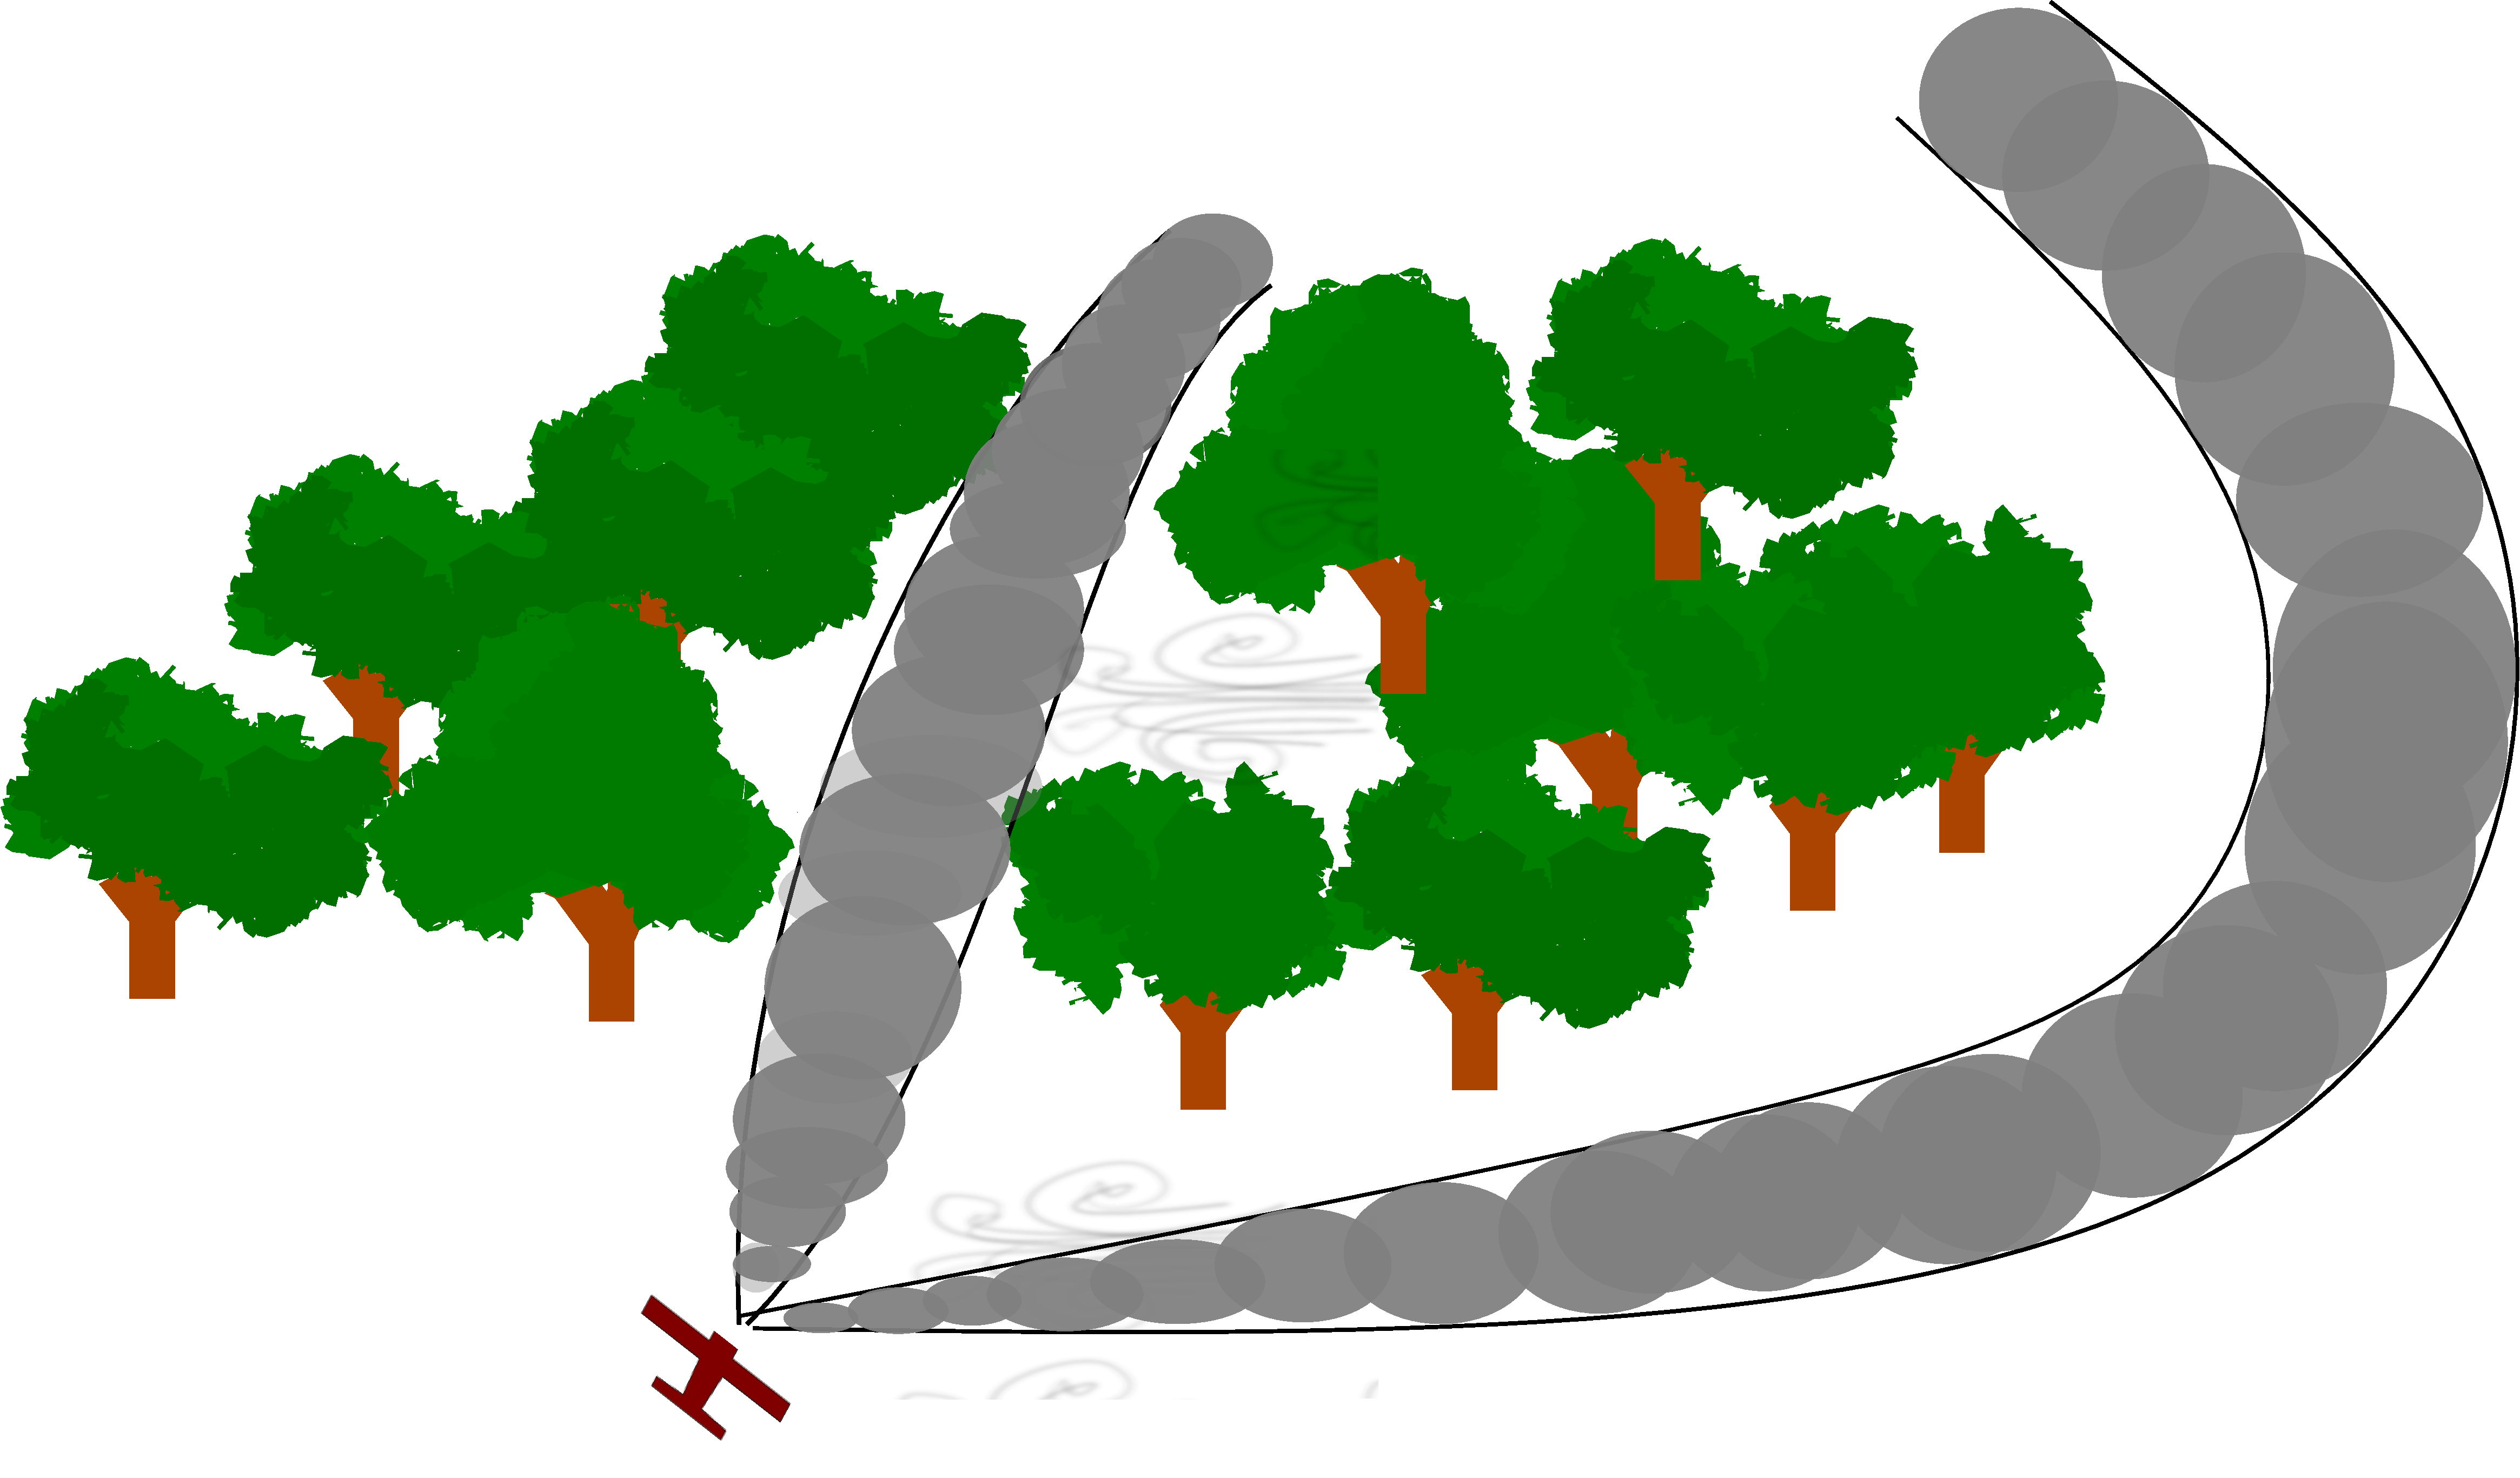
\includegraphics[width=.8\textwidth]{figures/experiments/aggressive-maneuver}
  \caption[Advantages of explicitly reasoning about uncertainty]{A planner that
    is guaranteed to not collide might as well go straight through the opening
    in the forest, instead of the long way around an obstacle.}
  \label{fig:aggressive-maneuver}
\end{figure}

In general planning is harder for a nonlinear and non-holonomic vehicle.
Especially when uncertainty is added to the model. In this case a lot of
planners simply choose to ignore these error sources and instead apply
heuristics such as maximizing the distance to the obstacles in the environment.
However, this adds the disadvantage that the plans can become overly
conservative. Explicitly handling the uncertainties at the planning stage
enables the planner to employ more aggressive maneuvers, such as flying through
two trees that are close together, as opposed to flying around the entire grove,
when tasked with flying through a strip of forest. Because of this, flying
straight through is an acceptable maneuver for a planner that has guarantees on
the whereabouts of the dynamical system, and hence is not afraid of collisions,
even when close to an obstacle. An example of this can be seen in
\cref{fig:aggressive-maneuver}. In this thesis this confidence in planning is
enabled by the calculation of \textit{robust motion primitives} through the
\ac{SOS} framework developed in \cref{sec:funnels}.

As it currently stands the current implementation of the \rrtfunnel{} algorithm
handles uncertainty only in the position of the dynamical system, but can be
easily extended to handle uncertainty in input and speed as well by employing a
different dynamical model. Handling uncertainties in the environment is not
possible with the current approach. Abstractly, the algorithm is built up from
two main parts:

\subparagraph{i)} One, is the calculation of \textit{robust motion primitives},
which allows the global motion planner to remain completely oblivious to these
difficulties, and hence act as though there were no uncertainties during the
planning stage. This means that a lot of the difficulty in planning is handled
during the off-line phase of generating the robust motion primitives themselves.
The advent of \ac{SOS} programming enables a numerical search for a Lyapunov
function to verify the convergence of the nonlinear feedback system. The
one-level subset of the Lyapunov function is then used as the reachable set of
the dynamical system. Adding uncertainty to the verification is made through the
addition of extra constraints to the \ac{SOS} program definition. Through
formulating the search for a \textit{Lyapunov function} for the system as a
\ac{SOS} program, the trajectories are extended to so called `funnels', which
incorporate all the states the system can be in during a given time frame --
even in the face of uncertainties. In the literature this is referred to as a
\textit{finite time reachable set}, meaning that if the calculations are
correct, it contains all the states that the system can evolve to in a given
time frame from a set of initial conditions under the influence of a bounded
uncertainty term.


\subparagraph{ii)} Second, the aforementioned funnels are then employed as
\textit{motion primitives} for the global \ac{RRT} motion planning algorithm.
Meaning that they all encode a discrete action. For the dynamical system in this
thesis, which is a simple unicycle model, the motion primitives can be a simple
`turn-left', `turn-right', or `go-straight' motion. Thus by stacking one motion
primitive after the other, one is able to create a plan, and by extension build
one long motion primitive through the overarching environment. With the motion
primitives being robust to uncertainty, these plans are in theory guaranteed to
be collision-free. The reason the theory employed here does not necessarily
apply to the real world is that most noise is not bounded in the real world, and
hence the assumptions made may not be correct. The \ac{RRT} algorithm can handle
large state spaces and differential constraints. However, it is not able to
directly reason about uncertainty and feedback during the planning stage. It is
therefore that this thesis seeks to combine the \ac{SOS} programming framework
in order to generate robust motion primitives for the \ac{RRT} algorithm. The
planner will then use these primitives during the planning stage, and hence act
like a normal \ac{RRT} planning algorithm, yet handle all the difficulties of
uncertainty and feedback, as this is contained in the motion primitives employed
as branches in the planning tree.

\begin{figure}
  \centering
  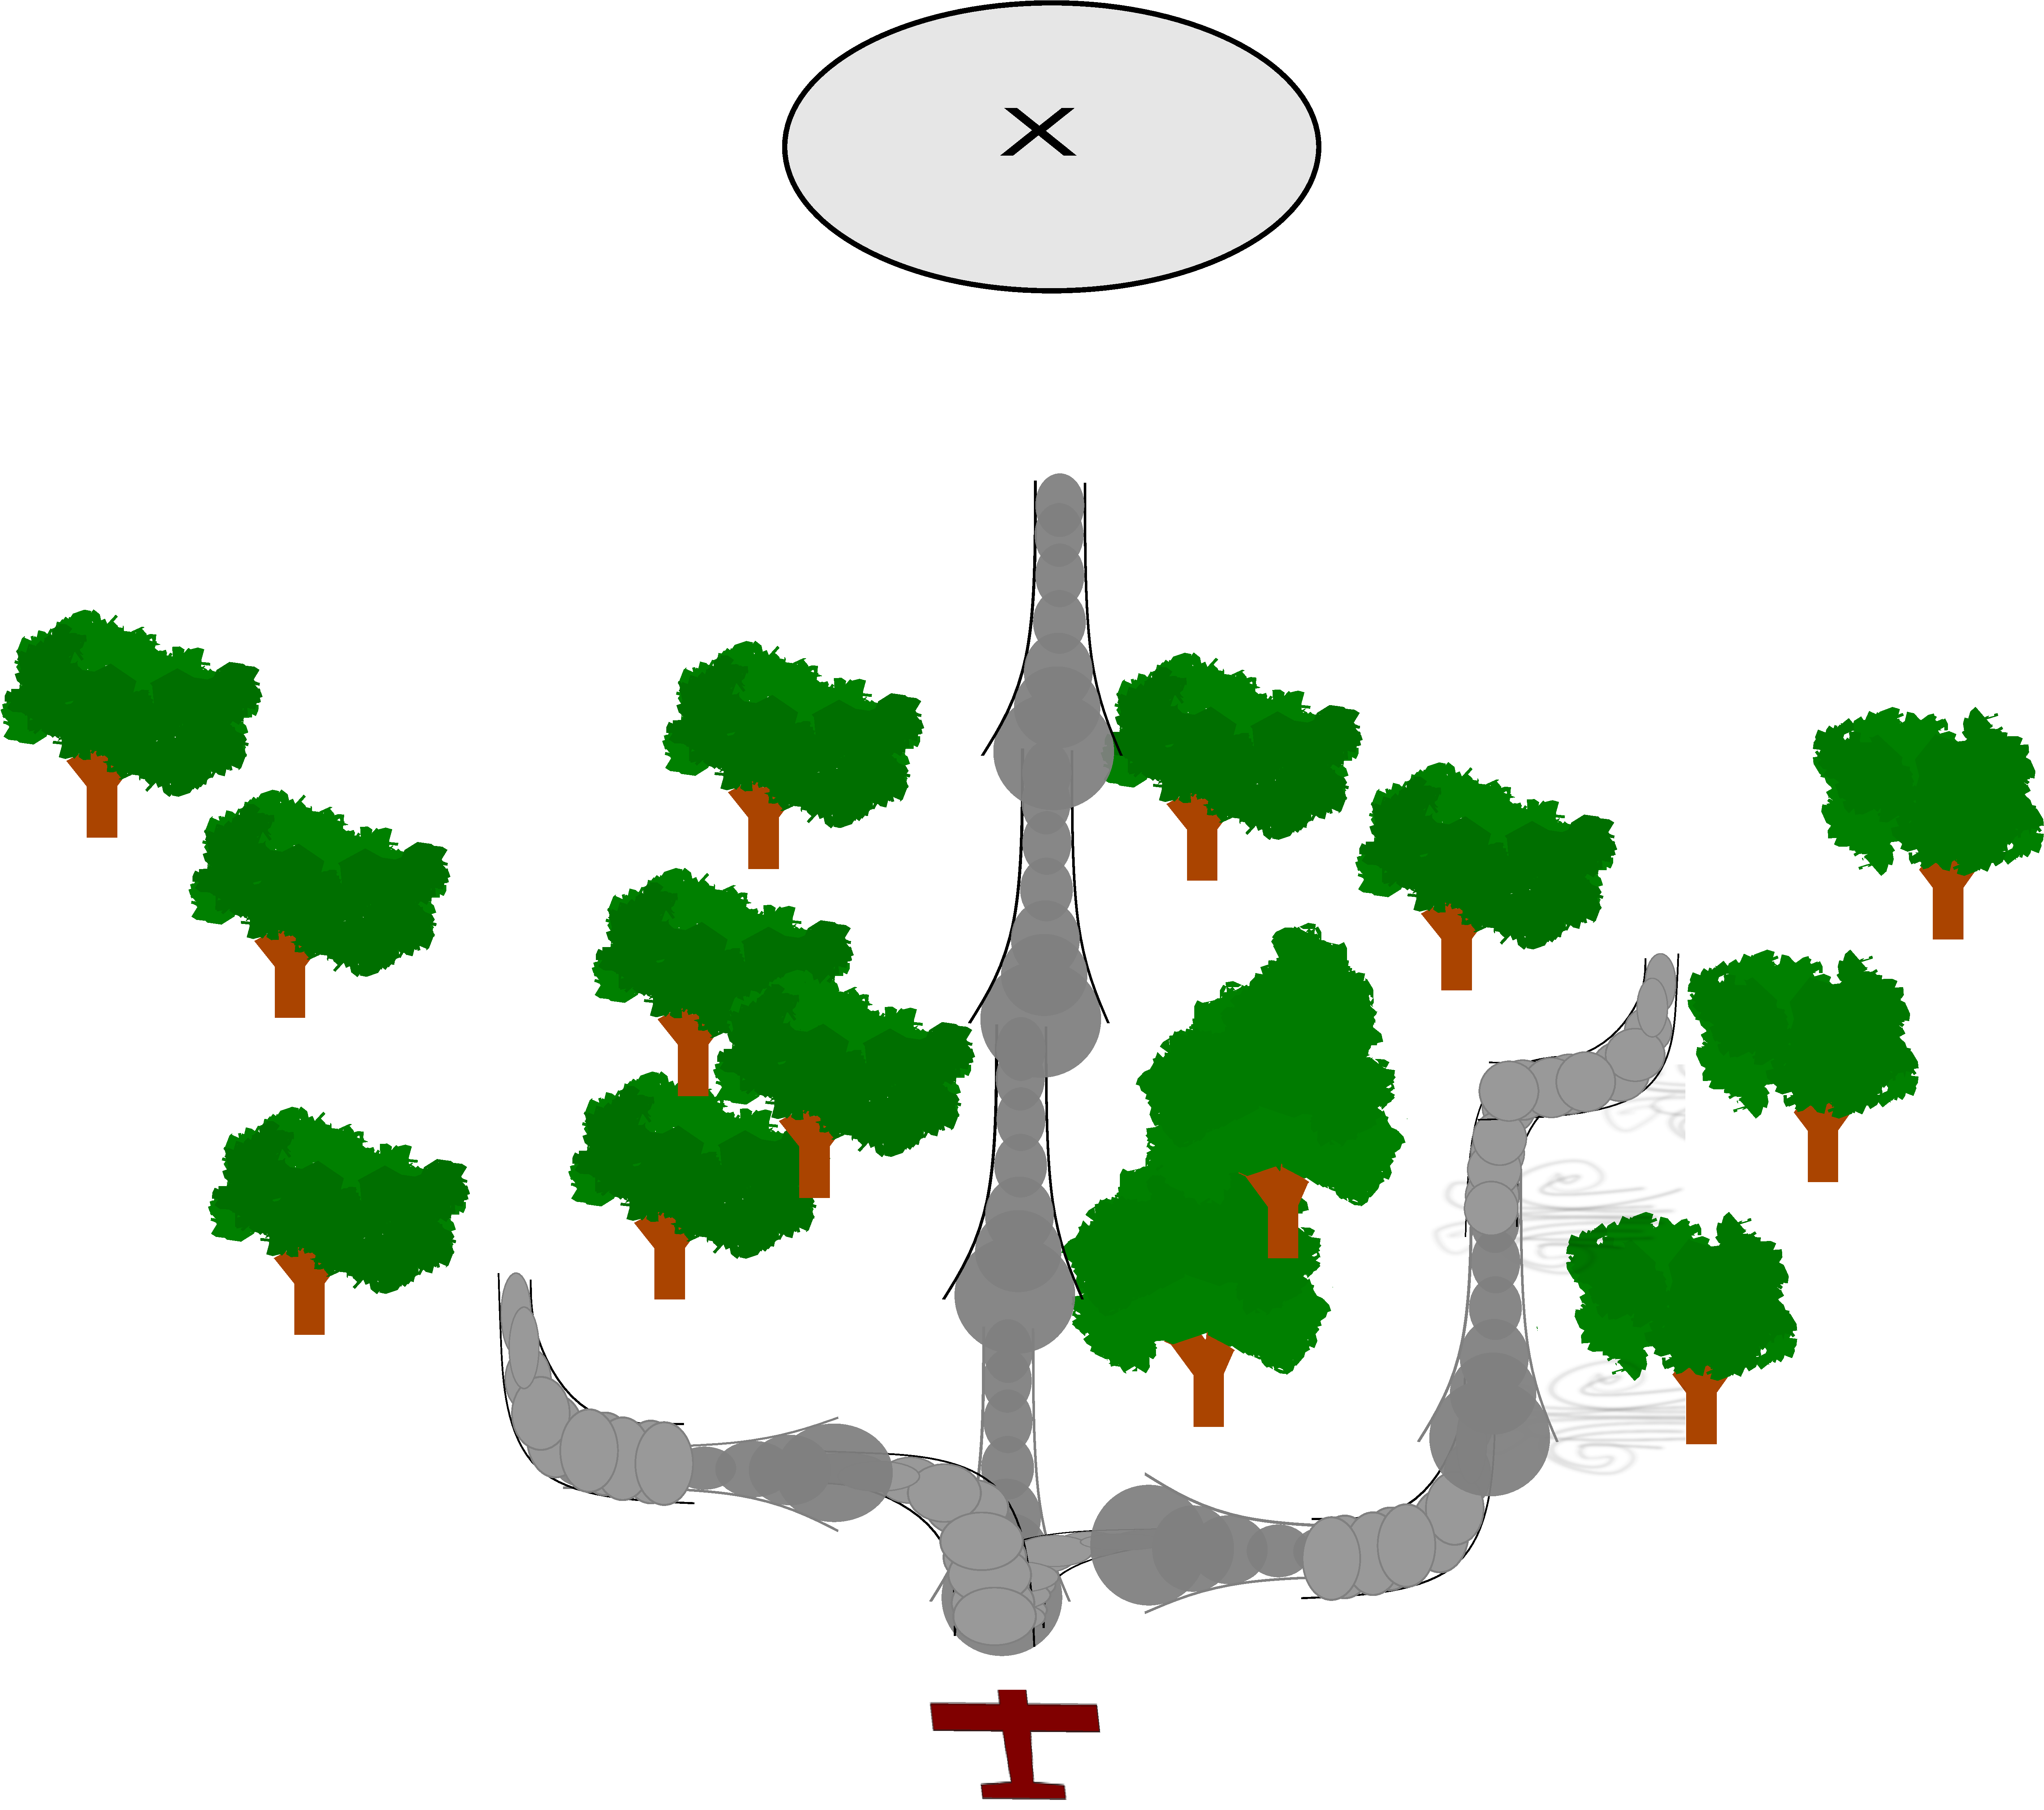
\includegraphics[width=.8\textwidth]{figures/experiments/experiment-airplane-strip}
  \caption[The experiment setup visualized]{An illustration of the experiment
    setup, showing how the \rrtfunnel{} algorithm builds a tree of funnels to
    find a safe path through a strip of forest.}
  \label{fig:experiments-cartoon}
\end{figure}

\paragraph{Experiments}
This theoretical robustness guarantee is later put to the test in simulated
experimental runs through a strip of forest of some density meant to make
planning difficult, along with a cross-wind given to the system as noise. A
cartoon of the experiment environment can be seen in
\cref{fig:experiments-cartoon}. Hence the airplane is constantly faced with a
positional offset, and is forced to deal with this as best as it is able to
during execution of the plan. As is shown, the robustness guarantees provided by
the Lyapunov functions found through the \ac{SOS} programs formulated do provide
safe traversal through the environment, as opposed to a planner which does not.

\section{Problem Description}

Current motion planning algorithms do not in the general case handle the problem
of uncertainty during planning. This is not optimal, in that all real-world
motion planning problems have to handle uncertainties. Therefore, this thesis
focus is on developing a motion planning algorithm that is robust to
uncertainty, and verifying the safe traversal of the algorithm through
simulation.
% \subsection{What has been done by others}

% The two main parts of the \rrtfunnel{} algorithm is the funnel generation
% framework through \ac{SOS} programming. Although this is used in a lot of
% different research, the strand that this thesis is based upon is a series of
% papers~\cite{Tobenkin_2011,tedrakeLQRtreesFeedbackMotion2009,majumdarRobustOnlineMotion2013,majumdarFunnelLibrariesRealtime2017,ahmadi2014dsos}
% with the main focus being on \cite{majumdarFunnelLibrariesRealtime2017}. The
% second part is based on~\textcite{article} and the \ac{RRT} motion planning
% algorithm, which is a simple algorithm that seeks to build a random tree that
% quickly expands deeply into the state space, and due to its random nature is
% good at avoiding local extrema.

\subsection{Scientific Contributions}

The contribution of this thesis is the combination of the \ac{RRT} motion
planning algorithm with the safe traversal guarantees provided by the \ac{SOS}
programming framework. The finite time reachable sets produced by the \ac{SOS}
program are then employed as robust motion primitives to the \ac{RRT} motion
planner, enabling it to create a tree of safe maneuvers while it searches for a
path to the goal for a nonlinear dynamical system -- even in the face of
uncertainty.


\section{Outline}

The rest of the thesis is organized as follows:
\begin{description}

\item[\cref{chp:survey-of-papers}] provides a survey of current motion planning
  research, with a focus on handling uncertainty in the environment, the system
  state and the surrounding environment.    

\item[\cref{chp:preliminaries}] provides introductory theory. First to motion
  planning as a general topic, and then introduces the funnel generation theory
  through \ac{SOS} programming framework. Finally it develops the basic theory
  needed for understanding the inner workings of the \ac{RRT} algorithm.
    
\item[\cref{chp:method}] develops the \rrtfunnel{} algorithm through two parts.
  Firstly it develops robust motion primitives through the \ac{SOS} programming
  framework. Then it develops the needed heuristics and sampling distribution
  for the \ac{RRT} motion planner and then incorporates the funnels from the
  first part as the extension operators to the tree that the \ac{RRT} algorithm
  builds through the configuration space.
    
\item[\cref{chp:experiments}] contains the description of how to create and
  setup the experiment environment and the benchmark planner that is used in
  comparing the performance of the \rrtfunnel{} algorithm.

\item[\cref{chp:discussion}] gives a discussion of the results, and references
  future work on the problem.

\item[\cref{sec:first-app}] gives a basic introduction to the theory of \ac{SOS}
  verification for dynamical systems.

\item[\cref{AppendixB}] contains some code examples from the code for the
  implementation of the \rrtfunnel{} algorithm. The rest of which can be found
  in~\cite{MasterThesisCode2019}.

\end{description}


